\chapter{Desarrollo Teórico y Simulaciones}

\section{Determinación de los Parámetros del Circuito Equivalente}

Los parámetros del modelo eléctrico equivalente de un transformador monofásico se obtienen clásicamente a partir de dos
ensayos normalizados realizados desde el lado de alta tensión (AT): el ensayo de vacío y el ensayo de cortocircuito.

A partir de los datos de placa del transformador:
\begin{gather*}
    S_N = \SI{100}{\kilo\volt\ampere} \\
    V_{1N} = \SI{3000}{\volt} \quad \text{(Lado AT)} \\
    V_{2N} = \SI{220}{\volt} \quad \text{(Lado BT)}
\end{gather*}
Se calculan las corrientes nominales primaria ($I_{1N}$) y secundaria ($I_{2N}$):
\begin{equation*}
    I_{1N} = \frac{S_N}{V_{1N}} = \frac{\SI{100}{\kilo\volt\ampere}}{\SI{3000}{\volt}} = \SI{33,33}{\ampere}
\end{equation*}
\begin{equation*}
    I_{2N} = \frac{S_N}{V_{2N}} = \frac{\SI{100}{\kilo\volt\ampere}}{\SI{220}{\volt}} = \SI{454,55}{\ampere}
\end{equation*}

La relación de transformación teórica ($m$) se define como:
\begin{equation*}
    m = \frac{V_{1N}}{V_{2N}} = \frac{\SI{3000}{\volt}}{\SI{220}{\volt}} = 13,636
\end{equation*}

\subsection{Ensayo de Vacío (Lado AT)}
El ensayo de vacío permite determinar los parámetros de la rama paralela o magnetizante del transformador: la
resistencia de pérdidas en el hierro ($R_{Fe}$) y la reactancia magnetizante ($X_\mu$). Los valores medidos en el ensayo, registrados a través del simulador (ver Figura~\ref{fig.anexo:vacio} del Anexo~\ref{sec.anexo:capturas}), son:
\begin{gather*}
    V_0 = \SI{3000}{\volt} \\
    I_0 = \SI{0,64}{\ampere} \\
    P_0 = \SI{830}{\watt}
\end{gather*}
La componente activa ($I_{Fe}$) de la corriente de vacío, asociada a las pérdidas en el núcleo, se determina como:
\begin{equation*}
    I_{Fe} = \frac{P_0}{V_0} = \frac{\SI{830}{\watt}}{\SI{3000}{\volt}} = \SI{0,2766}{\ampere}
\end{equation*}
A partir de ella, se obtiene por la ley de Ohm la resistencia que modela las pérdidas en el hierro ($R_{Fe}$):
\begin{equation*}
    R_{Fe} = \frac{V_0}{I_{Fe}} = \frac{\SI{3000}{\volt}}{\SI{0,2766}{\ampere}} = \SI{10843}{\ohm}
\end{equation*}

La componente reactiva o magnetizante ($I_\mu$) de la corriente de vacío se obtiene utilizando la relación trigonométrica
de Pitágoras sobre el triángulo de corrientes:
\begin{equation*}
    I_\mu = \sqrt{I_0^2 - I_{Fe}^2} = \sqrt{(\SI{0,64}{\ampere})^2 - (\SI{0,2766}{\ampere})^2} = \SI{0,5771}{\ampere}
\end{equation*}
De allí, aplicando la ley de Ohm, se calcula la reactancia magnetizante ($X_\mu$):
\begin{equation*}
    X_\mu = \frac{V_0}{I_\mu} = \frac{\SI{3000}{\volt}}{\SI{0,5771}{\ampere}} = \SI{5198,3}{\ohm}
\end{equation*}

\subsection{Ensayo de Cortocircuito (Lado AT)}
Este ensayo permite obtener los parámetros en serie del transformador, que modelan la caída de tensión interna y las
pérdidas en los devanados primario y secundario. Se realiza aplicando una tensión reducida de cortocircuito ($V_{cc}$)
hasta alcanzar la corriente nominal en el primario, obteniéndose los valores medidos en el simulador (ver la captura nominal en la Figura~\ref{fig.anexo:cc_controlado_77V} del Anexo~\ref{sec.anexo:capturas}):
\begin{gather*}
    V_{cc} = \SI{77}{\volt} \\
    I_{cc} = I_{1N} = \SI{33,33}{\ampere} \\
    P_{cc} = \SI{650}{\watt}
\end{gather*}

La impedancia de cortocircuito total ($Z_{cc}$) y la resistencia de cortocircuito ($R_{cc}$) son:
\begin{equation*}
    Z_{cc} = \frac{V_{cc}}{I_{cc}} = \frac{\SI{77}{\volt}}{\SI{33,33}{\ampere}} = \SI{2,31}{\ohm}
\end{equation*}
\begin{equation*}
    R_{cc} = \frac{P_{cc}}{I_{cc}^2} = \frac{\SI{650}{\watt}}{(\SI{33,33}{\ampere})^2} = \SI{0,585}{\ohm}
\end{equation*}

La reactancia de dispersión equivalente de cortocircuito ($X_{cc}$) es:
\begin{equation*}
    X_{cc} = \sqrt{Z_{cc}^2 - R_{cc}^2} = \sqrt{(\SI{2,31}{\ohm})^2 - (\SI{0,585}{\ohm})^2} = \SI{2,23}{\ohm}
\end{equation*}

Para modelar por separado los devanados en el simulador de Aula Moisan, se distribuyen los parámetros de forma
simétrica entre el primario y el secundario referido:
\begin{equation*}
    R_p = R'_s = \frac{R_{cc}}{2} = \SI{0,2925}{\ohm}
\end{equation*}
\begin{equation*}
    X_{dp} = X'_{ds} = \frac{X_{cc}}{2} = \SI{1,115}{\ohm}
\end{equation*}


\section{Impedancia de Carga y Discrepancias en la Simulación}

\subsection{Cálculo Teórico Correcto de la Impedancia de Carga}
De acuerdo con las consignas físicas y la teoría de circuitos acoplados magnéticamente, para un porcentaje de carga
especificado por la fracción de carga $C$, la impedancia de carga en el secundario (BT) a tensión nominal es:
\begin{equation}
    Z_c = \frac{V_{2N}^2}{S_N \cdot C}
\end{equation}
Para trasladar esta impedancia al primario (lado de AT), se multiplica por el cuadrado de la relación de transformación:
\begin{equation*}
    Z'_c = Z_c \cdot m^2 = Z_c \cdot (13,636)^2
\end{equation*}
Para factores de potencia diferentes a la unidad, el ángulo de la carga ($\theta_Z$) se determina como:
\begin{equation}
    \theta_Z = \pm\arccos(f_p)
\end{equation}
siendo positivo para cargas inductivas y negativo para capacitivas.

Los valores teóricos correctos de impedancia de carga se resumen en la Tabla~\ref{tab.ej1:impedancias_teoricas}.

\begin{table}[!ht]
    \centering
    \begin{tabular}{|c|c|c|c|c|}
        \hline
        Condición & C & $Z_c$ BT [\si{\ohm}] & $Z'_c$ AT [\si{\ohm}] & $\theta_Z$ [$^\circ$] \\
        \hline
        Vacío & - & $\infty$ & $\infty$ & $0$ \\
        Carga $\SI{25}{\percent}$ - $f_p = 1$ & $0,25$ & $1,936$ & $360,0$ & $0$ \\
        Carga $\SI{50}{\percent}$ - $f_p = 1$ & $0,50$ & $0,968$ & $180,0$ & $0$ \\
        Carga $\SI{75}{\percent}$ - $f_p = 1$ & $0,75$ & $0,645$ & $120,0$ & $0$ \\
        Carga $\SI{100}{\percent}$ - $f_p = 1$ & $1,00$ & $0,484$ & $90,0$ & $0$ \\
        Carga $\SI{100}{\percent}$ - $f_p = 0,8$ ind & $1,00$ & $0,484$ & $90,0$ & $+36,87$ \\
        Carga $\SI{100}{\percent}$ - $f_p = 0,8$ cap & $1,00$ & $0,484$ & $90,0$ & $-36,87$ \\
        \hline
    \end{tabular}
    \caption{Cálculo de impedancias de carga teóricas referidas al primario ($V_{2N} = \SI{220}{\volt}, m = 13,636$).}
    \label{tab.ej1:impedancias_teoricas}
\end{table}

\section{Tablas de Resultados del Simulador}

Se transcriben a continuación los valores numéricos obtenidos de las variables indicadas en las capturas del simulador.

\subsection{Ensayos de Vacío y Carga}
La Tabla \ref{tab.ej1:resultados_simulador_carga} recopila los resultados de las simulaciones a tensión primaria nominal
($V_p = \SI{3000}{\volt}$) para los distintos estados de carga simulados. Las capturas de pantalla de la interfaz del simulador para cada uno de los puntos ensayados se presentan en las Figuras~\ref{fig.anexo:grupo_carga_resistiva} (para $f_p = 1,0$), \ref{fig.anexo:grupo_carga_inductiva} (para $f_p = 0,8$ inductivo) y \ref{fig.anexo:grupo_carga_capacitiva} (para $f_p = 0,8$ capacitivo) del Anexo~\ref{sec.anexo:capturas}.

\begin{table}[!ht]
    \centering
    \resizebox{\textwidth}{!}{
    \begin{tabular}{|c|c|c|c|c|c|c|c|c|c|}
        \hline
        Condición & C & $Z'_c$ [\si{\ohm}] & $\theta_Z$ [$^\circ$] & $I_p$ [\si{\ampere}] & $\theta_{Ip}$ [$^\circ$] & $V_s$ [\si{\volt}] & $P_{abs}$ [\si{\watt}] & $P_{Fe}$ [\si{\watt}] & $\eta$ [\%] \\
        \hline
        Vacío & - & $1\text{E+}99$ & $0$ & $0,64$ & $-64,39$ & $220,05$ & $829,75$ & $829,63$ & $\approx 0$ \\
        \hline
        Carga $\SI{25}{\percent}$ - $f_p = 1$ & $0,25$ & $360$ & $0$ & $8,62$ & $-4,19$ & $219,69$ & $25776,20$ & $828,26$ & $96,62$ \\
        Carga $\SI{50}{\percent}$ - $f_p = 1$ & $0,50$ & $180$ & $0$ & $16,90$ & $-2,66$ & $219,32$ & $50636,10$ & $826,85$ & $98,04$ \\
        Carga $\SI{75}{\percent}$ - $f_p = 1$ & $0,75$ & $120$ & $0$ & $25,16$ & $-2,37$ & $218,95$ & $75404,20$ & $825,40$ & $98,42$ \\
        Carga $\SI{100}{\percent}$ - $f_p = 1$ & $1,00$ & $90$ & $0$ & $33,39$ & $-2,39$ & $218,56$ & $100076,00$ & $823,91$ & $98,53$ \\
        \hline
        Carga $\SI{25}{\percent}$ - $f_p = 0,8$ ind & $0,25$ & $360$ & $+36,87$ & $8,86$ & $-39,00$ & $218,95$ & $20659,50$ & $825,48$ & $95,80$ \\
        Carga $\SI{50}{\percent}$ - $f_p = 0,8$ ind & $0,50$ & $180$ & $+36,87$ & $17,06$ & $-38,30$ & $217,86$ & $40174,10$ & $821,37$ & $97,55$ \\
        Carga $\SI{75}{\percent}$ - $f_p = 0,8$ ind & $0,75$ & $120$ & $+36,87$ & $25,19$ & $-38,21$ & $216,77$ & $59378,10$ & $817,29$ & $98,01$ \\
        Carga $\SI{100}{\percent}$ - $f_p = 0,8$ ind & $1,00$ & $90$ & $+36,87$ & $33,23$ & $-38,26$ & $215,70$ & $78276,20$ & $813,24$ & $98,15$ \\
        \hline
        Carga $\SI{25}{\percent}$ - $f_p = 0,8$ cap & $0,25$ & $360$ & $-36,87$ & $8,25$ & $+32,16$ & $220,58$ & $20958,50$ & $831,62$ & $95,84$ \\
        Carga $\SI{50}{\percent}$ - $f_p = 0,8$ cap & $0,50$ & $180$ & $-36,87$ & $16,63$ & $+34,01$ & $221,10$ & $41360,60$ & $833,57$ & $97,59$ \\
        Carga $\SI{75}{\percent}$ - $f_p = 0,8$ cap & $0,75$ & $120$ & $-36,87$ & $25,17$ & $+34,39$ & $221,26$ & $62024,9$ & $835,49$ & $98,05$ \\
        Carga $\SI{100}{\percent}$ - $f_p = 0,8$ cap & $1,00$ & $90$ & $-36,87$ & $33,53$ & $+34,42$ & $222,13$ & $82980,10$ & $837,38$ & $98,20$ \\
        \hline
    \end{tabular}
    }
    \caption{Resultados del simulador para vacío y carga ($V_p = \SI{3000}{\volt}, rt = 13,636$).}
    \label{tab.ej1:resultados_simulador_carga}
\end{table}

\subsection{Ensayo de Cortocircuito Controlado}
El ensayo de cortocircuito controlado consiste en aplicar tensión reducida en el primario con el secundario en
cortocircuito ($Z'_c = \SI{0}{\ohm}, \theta_Z = 0$) hasta alcanzar la corriente nominal. La
Tabla~\ref{tab.ej1:resultados_simulador_cc_controlado} muestra el barrido de tensión. Las capturas correspondientes a todo el barrido de tensión simulado (de \SI{0}{\volt} a \SI{77}{\volt}) se detallan en la Figura~\ref{fig.anexo:cc_barrido} del Anexo~\ref{sec.anexo:capturas}.

\begin{table}[!ht]
    \centering
    \caption{Resultados del ensayo de cortocircuito controlado ($Z'_c = \SI{0}{\ohm}$).}
    \label{tab.ej1:resultados_simulador_cc_controlado}
    \begin{tabular}{|c|c|c|}
        \hline
        $V_p$ [\si{\volt}] & $I_p$ [\si{\ampere}] & $P_{abs}$ [\si{\watt}] \\
        \hline
        $0$ & $0,00$ & $0,00$ \\
        $10$ & $4,34$ & $11,01$ \\
        $20$ & $8,68$ & $44,03$ \\
        $30$ & $13,01$ & $99,08$ \\
        $40$ & $17,35$ & $176,14$ \\
        $50$ & $21,69$ & $275,22$ \\
        $60$ & $26,03$ & $396,31$ \\
        $70$ & $30,37$ & $539,42$ \\
        $77$ & $33,40$ & $652,70$ \\
        \hline
    \end{tabular}
\end{table}

Alcanzada la tensión reducida $V_{cc} = \SI{77}{\volt}$, se verifica que la corriente primaria $I_p =
\SI{33,40}{\ampere}$ es muy cercana a $I_{1N} = \SI{33,33}{\ampere}$ y la potencia activa es $P_{abs} =
\SI{652,70}{\watt}$ (cercana a $P_{cc} = \SI{650}{\watt}$ del ensayo original).

\subsection{Ensayo de Cortocircuito Franco}
El cortocircuito franco representa la condición de falla al aplicar la tensión nominal completa con impedancia de carga
nula (ver captura del simulador en la Figura~\ref{fig.anexo:cc_franco} del Anexo~\ref{sec.anexo:capturas}):
\begin{gather*}
    I_p = \SI{1301,42}{\ampere} \quad V_s = \SI{0}{\volt}\\[6pt]
    P_{abs} = \SI{990,78}{\kilo\watt} \quad \eta = \SI{0}{\percent}
\end{gather*}

\section{Gráficos de Comportamiento}

A partir de los datos registrados en el simulador, se confeccionan las gráficas para analizar el comportamiento. En la
Figura \ref{fig.ej1:plot_regulacion} se presentan las curvas de regulación de la tensión secundaria en función de la
fracción de carga para los distintos factores de potencia, mientras que en la Figura~\ref{fig.ej1:plot_rendimiento} se
ilustra la curva de rendimiento del transformador monofásico simulado.

\begin{figure}[!ht]
    \centering
    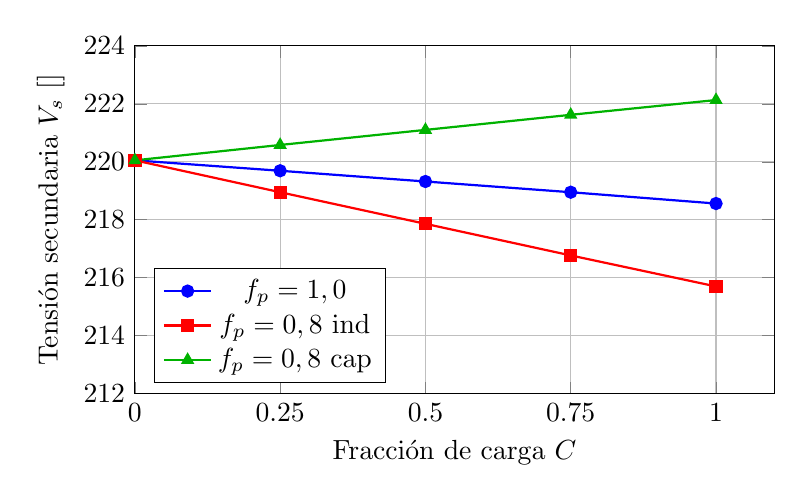
\begin{tikzpicture}
  \begin{axis}[
      xlabel={Fracción de carga $C$},
      ylabel={Tensión secundaria $V_s$ [\si{\volt}]},
      xmin=0, xmax=1.1,
      ymin=212, ymax=224,
      xtick={0, 0.25, 0.5, 0.75, 1},
      ytick={212, 214, 216, 218, 220, 222, 224},
      legend pos=south west,
      grid=major,
      width=0.8\textwidth,
      height=6cm
    ]
    % Carga resistiva (fp = 1)
    \addplot[color=blue, mark=*, thick] coordinates {
      (0, 220.05)
      (0.25, 219.69)
      (0.50, 219.32)
      (0.75, 218.95)
      (1.00, 218.56)
    };
    \addlegendentry{$f_p = 1,0$}

    % Carga inductiva (fp = 0.8 ind)
    \addplot[color=red, mark=square*, thick] coordinates {
      (0, 220.05)
      (0.25, 218.95)
      (0.50, 217.86)
      (0.75, 216.77)
      (1.00, 215.70)
    };
    \addlegendentry{$f_p = 0,8$ ind}

    % Carga capacitiva (fp = 0.8 cap)
    \addplot[color=green!70!black, mark=triangle*, thick] coordinates {
      (0, 220.05)
      (0.25, 220.58)
      (0.50, 221.10)
      (0.75, 221.62)
      (1.00, 222.13)
    };
    \addlegendentry{$f_p = 0,8$ cap}
  \end{axis}
\end{tikzpicture}

    \caption{Curvas de regulación en función de ($C$) para diferentes f.d.p.}
    \label{fig.ej1:plot_regulacion}
\end{figure}

\begin{figure}[!ht]
    \centering
    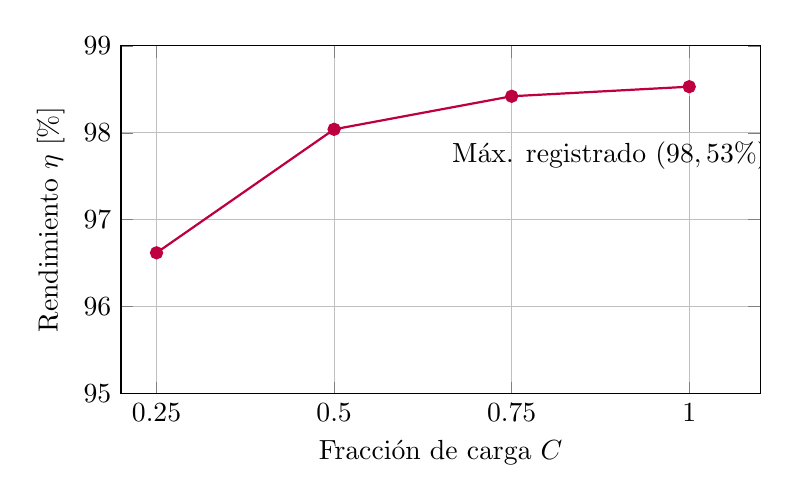
\begin{tikzpicture}
  \begin{axis}[
      xlabel={Fracción de carga $C$},
      ylabel={Rendimiento $\eta$ [\%]},
      xmin=0.2, xmax=1.1,
      ymin=95, ymax=99,
      xtick={0.25, 0.5, 0.75, 1},
      ytick={95, 96, 97, 98, 99},
      grid=major,
      width=0.8\textwidth,
      height=6cm
    ]
    \addplot[color=purple, mark=*, thick] coordinates {
      (0.25, 96.62)
      (0.50, 98.04)
      (0.75, 98.42)
      (1.00, 98.53)
    };
    
    \node[pin=270:{Máx. registrado ($98,53\%$) en $C=1,00$}] at (axis cs:1.00, 98.53) {};
  \end{axis}
\end{tikzpicture}

    \caption{Rendimiento ($\eta$) del transformador simulado en función de ($C$) para $f_p = 1$.}
    \label{fig.ej1:plot_rendimiento}
\end{figure}
